\documentclass{article}[18pt]
\ProvidesPackage{format}
%Page setup
\usepackage[utf8]{inputenc}
\usepackage[margin=0.7in]{geometry}
\usepackage{parselines} 
\usepackage[english]{babel}
\usepackage{fancyhdr}
\usepackage{titlesec}
\hyphenpenalty=10000

\pagestyle{fancy}
\fancyhf{}
\rhead{Sam Robbins}
\rfoot{Page \thepage}

%Characters
\usepackage{amsmath}
\usepackage{amssymb}
\usepackage{gensymb}
\newcommand{\R}{\mathbb{R}}

%Diagrams
\usepackage{pgfplots}
\usepackage{graphicx}
\usepackage{tabularx}
\usepackage{relsize}
\pgfplotsset{width=10cm,compat=1.9}
\usepackage{float}

%Length Setting
\titlespacing\section{0pt}{14pt plus 4pt minus 2pt}{0pt plus 2pt minus 2pt}
\newlength\tindent
\setlength{\tindent}{\parindent}
\setlength{\parindent}{0pt}
\renewcommand{\indent}{\hspace*{\tindent}}

%Programming Font
\usepackage{courier}
\usepackage{listings}
\usepackage{pxfonts}

%Lists
\usepackage{enumerate}
\usepackage{enumitem}

% Networks Macro
\usepackage{tikz}


% Commands for files converted using pandoc
\providecommand{\tightlist}{%
	\setlength{\itemsep}{0pt}\setlength{\parskip}{0pt}}
\usepackage{hyperref}

% Get nice commands for floor and ceil
\usepackage{mathtools}
\DeclarePairedDelimiter{\ceil}{\lceil}{\rceil}
\DeclarePairedDelimiter{\floor}{\lfloor}{\rfloor}

% Allow itemize to go up to 20 levels deep (just change the number if you need more you madman)
\usepackage{enumitem}
\setlistdepth{20}
\renewlist{itemize}{itemize}{20}

% initially, use dots for all levels
\setlist[itemize]{label=$\cdot$}

% customize the first 3 levels
\setlist[itemize,1]{label=\textbullet}
\setlist[itemize,2]{label=--}
\setlist[itemize,3]{label=*}

% Definition and Important Stuff
% Important stuff
\usepackage[framemethod=TikZ]{mdframed}

\newcounter{theo}[section]\setcounter{theo}{0}
\renewcommand{\thetheo}{\arabic{section}.\arabic{theo}}
\newenvironment{important}[1][]{%
	\refstepcounter{theo}%
	\ifstrempty{#1}%
	{\mdfsetup{%
			frametitle={%
				\tikz[baseline=(current bounding box.east),outer sep=0pt]
				\node[anchor=east,rectangle,fill=red!50]
				{\strut Important};}}
	}%
	{\mdfsetup{%
			frametitle={%
				\tikz[baseline=(current bounding box.east),outer sep=0pt]
				\node[anchor=east,rectangle,fill=red!50]
				{\strut Important:~#1};}}%
	}%
	\mdfsetup{innertopmargin=10pt,linecolor=red!50,%
		linewidth=2pt,topline=true,%
		frametitleaboveskip=\dimexpr-\ht\strutbox\relax
	}
	\begin{mdframed}[]\relax%
		\centering
		}{\end{mdframed}}



\newcounter{lem}[section]\setcounter{lem}{0}
\renewcommand{\thelem}{\arabic{section}.\arabic{lem}}
\newenvironment{defin}[1][]{%
	\refstepcounter{lem}%
	\ifstrempty{#1}%
	{\mdfsetup{%
			frametitle={%
				\tikz[baseline=(current bounding box.east),outer sep=0pt]
				\node[anchor=east,rectangle,fill=blue!20]
				{\strut Definition};}}
	}%
	{\mdfsetup{%
			frametitle={%
				\tikz[baseline=(current bounding box.east),outer sep=0pt]
				\node[anchor=east,rectangle,fill=blue!20]
				{\strut Definition:~#1};}}%
	}%
	\mdfsetup{innertopmargin=10pt,linecolor=blue!20,%
		linewidth=2pt,topline=true,%
		frametitleaboveskip=\dimexpr-\ht\strutbox\relax
	}
	\begin{mdframed}[]\relax%
		\centering
		}{\end{mdframed}}
\lhead{ADS - Part 4}
\lstset{language=C,
	basicstyle=\ttfamily,
	keywordstyle=\bfseries,
	showstringspaces=false,
	morekeywords={if, else, then, print, end, for, do, while},
	tabsize=4,
	mathescape=true,
	escapechar=£,
	numbers=left,
	stepnumber=1,
}

\usepackage{caption}
\DeclareCaptionFont{white}{\color{white}}
\DeclareCaptionFormat{listing}{\colorbox{gray}{\parbox{\textwidth}{#1#2#3}}}
\captionsetup[lstlisting]{format=listing,labelfont=white,textfont=white}

\begin{document}
\begin{center}
\underline{\huge String Matching}
\end{center}
\section{Problem Definition}
\begin{itemize}
	\item Given a (long) string T (over some (finite) alphabet $\Sigma$), and
	\item A (short) pattern P over the same alphabet (or subset)
	\item Find one or all occurrences of P in T, if any
\end{itemize}
For example:
T:acda\textcolor{red}{bdde}aa\textcolor{red}{bdde}\\
P:bdde
\section{Terminology}
\begin{itemize}
	\item Input is $T[1...n]$ and $P[1...m]$ with $m\leqslant n$
	\item Alphabet $\Sigma$ can be pretty much anything
	\item We say a pattern P occurs with shift s in T if
	\[ 
	0 \leq s \leq n-m \text { and } T[s+1, \ldots, s+m]=P[1 \ldots m]
	\]
	e.g.
	\begin{center}
		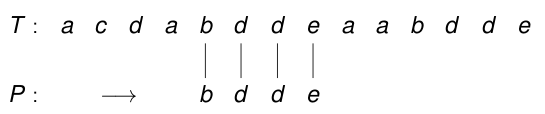
\includegraphics[scale=0.7]{Terminology}
	\end{center}
	Where we've got a shift of 4\\
	$T[5...8]=P[1...4]$ - shift 4\\
	$T[11...14]=P[1...4]$ - shift 10
	
\end{itemize}
\section{Shifts}
We say s is
\begin{itemize}
	\item A valid shift is P occurs with a shift s in T, and
	\item An invalid shift otherwise
\end{itemize}
In the example, 4 and 10 are valid shifts, all others are not.\\
\\
\textbf{Goal}: Find all occurrences of P in T(all valid shifts), as quickly as you can
\section{More Terminology}
Some notation:
\begin{itemize}
	\item $\Sigma$ is the alphabet, and $\Sigma^*$ ("Sigma Star") is the transitive closure, i.e., the set of all (finite) words that you can form using characters from $\Sigma$, e.g.
	\[ 
	\Sigma=\{0,1\} \Rightarrow \Sigma^{*}=\{\epsilon, 0,1,00,01,10,11,000, \ldots\}
	\]
	where $\epsilon$ denotes the empty word (the word of length 0)
	\item Length of a string $x$ is denoted by $|x|$
	\item Concatenation of string $x$ and $y$ is denoted $xy$, and $xy$'s length is $|xy|=|x|+|y|$
	\item Test $x\stackrel{?}{=}y$ can be done by comparing character by character starting at the leftmost position, and takes time $\Theta(t+1)$ with $t$ being length of longest string $z$ with $z  \sqsubset x$ and $z\sqsubset y$; notice the "+1" to handle case $t=0$ i.e. no common prefix
	\item Note that the notation $z\sqsubset x$ means z is the prefix of x
	\item Here t is the length of z (the longest match between the two strings)
\end{itemize}
\section{The naive algorithm}
Input string $T[1...n]$, pattern $P[1...m]$\\
Idea simple: just slide the pattern along the string and compare at each of the $n-m+1$ many positions
\begin{lstlisting}[caption=Naive Matcher]
for s=0 to n-m do
	if P[1...m]=T[s+1...s+m] then
		print "pattern occurs with shift s"
	end if
end for
\end{lstlisting}
Notice how we write the comparison as if it were a primitive operation(takes constant time), when in reality it isn't
\section{Example}
\begin{center}
	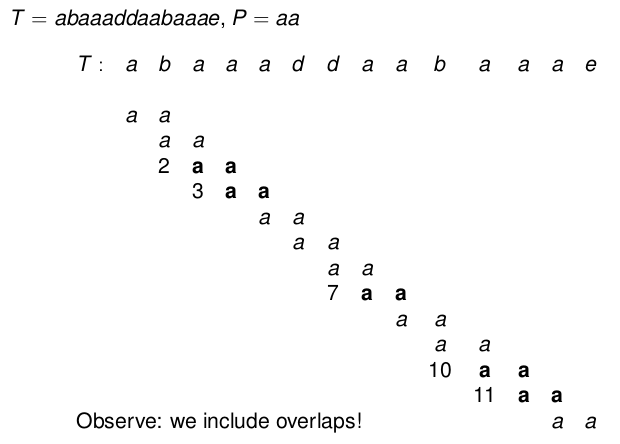
\includegraphics[scale=0.7]{Example}
\end{center}
Clearly running time $\mathcal{O}((n-m+1)\cdot m)$\\
This is tight in the sense that we have worst case instances that need precisely that (consider $T=a^n$ and $P=a^m$) = we need to compare the full pattern with whatever we find at each of the $n-m+1$ possible shifts\\
\\
Notice that this is
\begin{itemize}
	\item $\Theta(n^2)$ if $m\approx n/2$
	\item $\mathcal{O}(n)$ if $m=\mathcal{O}(1)$ or $m=n-\mathcal{O}(1)$
	\item $n\sqrt{n}=n^{3/2}$ if $m\approx \sqrt{n}$
\end{itemize}
This is not particularly good\\
\\
The biggest problems seems to be that we discard any information about previous comparisons when we move window to the right
\subsection{Example}
\begin{center}
	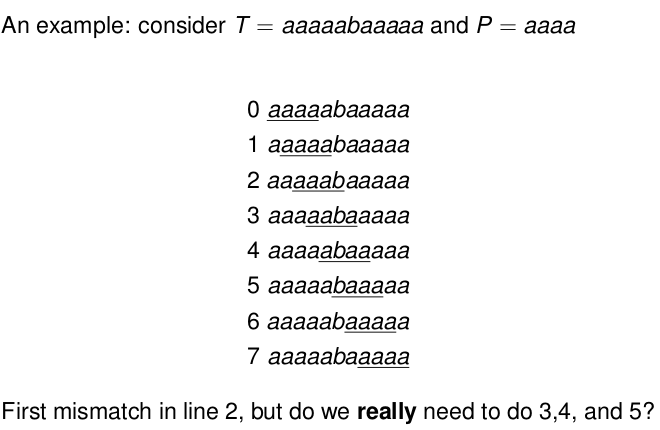
\includegraphics[scale=0.7]{Example1}
\end{center}
\section{The Rabin-Karp algorithm}
We introduce a second string-matching algorithm:
\begin{itemize}
	\item Still not best-possible
	\item Still same worst-case running time
	\item Still no "intelligent skipping"
	\item But in practice typically much better
\end{itemize}
\subsection{A useful idea}
\begin{itemize}
	\item Based on representation of substrings of length k as k-digit numbers
	\item That is, if our alphabet has size ten, represent string \texttt{61524} as decimal number 61,524
	\item This alone does of course not help - still need to make as many comparisons
	\item Extra idea: do calculations modulo some cleverly chosen number
	\item One of the very few examples where we need to think about "real world" performance
	\item Would normally assume that we can do arbitrary precision arithmetic in one step
	\item We will assume $\Sigma=\{0,1,2,3,4,5,6,7,8,9\}$
	\item Any other alphabet size is also possible, for example binary and hex
	\item Rabin-Karp does some preprocessing, and then the actual matching
	\item All the "better" string matching algorithms do some sort of preprocessing
	\item R-K needs $\Theta(m)$ time for preprocessing, and then worst case $\Theta((n-m+1)m)$ for matching - same as naive matcher
	\item However, much better "on average" - under certain assumptions
\end{itemize}
\section{Decimal Representations}
\begin{itemize}
	\item Given a pattern $P[1...m]$, denote by p its decimal value
	\item Likewise, given string $T[1...n]$, let $t_s$ denote decimal value of length-m substring $T=[s+1...s+m]$, for $s=0,1,...,n-m$
	\item Clearly, $T[s+1...s+m]=P$ iff $t_s=p$
	\item Therefore, s is a valid shift $\Leftrightarrow t_s=p$
\end{itemize}
What if we:
\begin{itemize}
	\item Could compute p in time $\mathcal{O}(m)$, and
	\item Could compute all the $t_s$ values in total time $\mathcal{O}(n-m+1)$ and
	\item Could compare $p$ with any given $t_s$ in constant time, then
	\item We'd have a $\mathcal{O}(m)+\mathcal{O}(n-m+1)=\mathcal{O}(n)$ algorithm
\end{itemize}
We can't... or can we?\\
We can certainly compute p from $P[1..m]$ in time $\mathcal{O}(m)$
\[ 
\begin{aligned} p=& P[m]+10 P[m-1]+100 P[m-2]+1000 P[m-3]+\cdots \\ & \cdots+10^{m-2} P[2]+10^{m-1} P[1] \\=& P[m]+10(P[m-1]+10 P[m-2]+100 P[m-3]+\cdots\\ & \cdots+10^{m-3} P[2]+10^{m-2} P[1] ) \\=& P[m]+10(P[m-1]+10(P[m-2]+10 P[m-3]+\cdots\\ & \vdots \\ &=P[m]+10(P[m-1]+10(P[m-2]+\cdots+10(P[2]+10 P[1]) \cdots)) \end{aligned}
\]
$\uparrow$ that all looks really scary, but it's just str to int conversion if you look at it\\
That is, use Horner's rule on $p(x)=\sum_{i=0}^{m-1}P[m-i]x^i$ in $x=10$ (compute from the right)\\
Can do the same for $t_0$ (from T[1..m]), the first m characters of T
\begin{itemize}
	\item We still need $t+1,t_2,..,t_{n-m}$
	\item We don't want to spend more than $\Theta(n-m)$ time for that, i.e. constant time for each $t_i, i\geqslant 1$
\end{itemize}
Simple, we can compute "new" $t_{s+1}$ based on $t_s$:
\begin{itemize}
	\item Consider e.g.
	\[ 
	\begin{array}{l}{15\underline{6274}5242133} \\ {156\underline{2745}242133}\end{array}
	\]
	i.e., focus on transition for $t_s=6274$ to $t_{s+1}=2745$ (with m=4)
	\item Notice that (when looking at strings) what we're really doing is
	\begin{itemize}
		\item Pushing the left-most 6 out, and
		\item Adding the 5 as new right most character
	\end{itemize}
	\item This corresponds to the arithmetic operation $10(6274-6\cdot 1000)+5$
	\item More generally, $t_{s+1}=10\left(t_{s}-10^{m-1} T[s+1]\right)+T[s+m+1]$
	\item Can precompute $10^{m-1}$ (it's always going to be $10^{m-1})$, then the execution takes constant time
\end{itemize}
\textbf{Summarising}
\begin{itemize}
	\item Thus, we can compute $p$ and $t_0$ in time $\Theta(m)$, and can compute all $t_1,...,t_{m-n}$ in total time $\Theta(n-m)$
	\item We can find all occurrences of P in T with $\Theta(m)$ for preprocessing of P, and $\Theta(n-m)$ for the matching
\end{itemize}
\textbf{But wait}
\begin{itemize}
	\item Surely, if m is very big, then $p$ and $t_i$ are very long numbers
	\item We wouldn't be able to store then in a computer word each
	\item Even if we used arbitrarily long integers (through, say, some class or other data structure in some library), it's be unrealistic to assume that we can do the actual arithmetic in constant time
\end{itemize}
\textbf{So what are we going to do}\\
Answer is quite simple, really: do everything, i.e., all arithmetic and such, modulo some (possibly much smaller) number q, so that every number fits into one computer word
\begin{itemize}
	\item Let's return to our example and chose $q=123$; note $h=10^3\mod 123=16$
	\item Consider the string 52424537454...
	\item Suppose we have computed $t_0$ (corresponds to 5242) as 76 ($5242 \mod 123=76$)
	\item Suppose we want to compute $t_1$; before we just did this:
	\[ 
	\begin{aligned} \mathbf{t}_{1}=t_{s+1} &=10\left(t_{s}-10^{m-1} T[s+1]\right)+T[s+m+1] \\ &=10\left(t_{0}-10^{m-1} T[1]\right)+T[0+4+1] \\ &=10(5242-1000 \cdot 5)+4 ] \\ &=10 \cdot 242+4=2420+4 \\ &=2424 \end{aligned}
	\]
	\item Observe that $2424\mod 123=87$
	\item Now working modulo q (recall $h=16, t_0=76$)
	\[ 
	\begin{aligned} \mathbf{t}_{1} &=\left(10\left(t_{0}-h T[s+1]\right)+T[s+m+1]\right) \bmod q \\ &=(10(76-16 \cdot 5)+4) \bmod 123 \\ &=(10(76-80)+4) \bmod 123 \\ &=(10(-4)+4) \bmod 123 \\ &=-36 \bmod 123=87 \end{aligned}
	\]
\end{itemize}
\textbf{That seems to work, or does it}
\begin{itemize}
	\item Consider T=62321462338294, P=3214, and q=123
	\item $3214\mod 123=16$
	\item If we compare the mod-123 values that we get for P and the substring of T at shift 2 (3214), then we get a match (which is OK)
	\item If we compare the mod-123 values that we get for P and the substring of T at shift 5 ($4623\mod 123=72$), then we get a mismatch (which is OK)
	\item If we compare the mod-123 values that we get for P and the substring of T at shift 9 (3829), then we get a match (which is not OK)
	\item In general, $t_s\neq p (\mod q)$ then we know for sure that $t_s\neq p$ (which is OK)
	\item However $t_s\equiv p (\mod q)$ does not necessarily imply $t_s=p$ (which is not OK)
\end{itemize}
\textbf{Ok, this doesn't seem to work that easily}
\begin{itemize}
	\item It looks as though we can use the text $t_s\stackrel{?}{\equiv}p(\mod q)$ really only as "heuristic"
	\item If the answer is no then we're fine
	\item If the answer is yes then we'll have to check in the old fashioned way and may get a false positive
	\item Hope that it doesn't happen too often, so that the extra cost isn't too high
	\item Make q large, so that we don't get "Too many collisions"
\end{itemize}
\end{document}